\subsection{Depth First Search}
\noindent Depth First Search (DFS) is a special case of backtracking search algorithm. The search starts from the root and proceeds to the farthest node before backtracking. The difference between this and the backtracking is that this stops the search once a goal is reached and does not care if it is not minimum.

\begin{figure}[H]
	\centering
	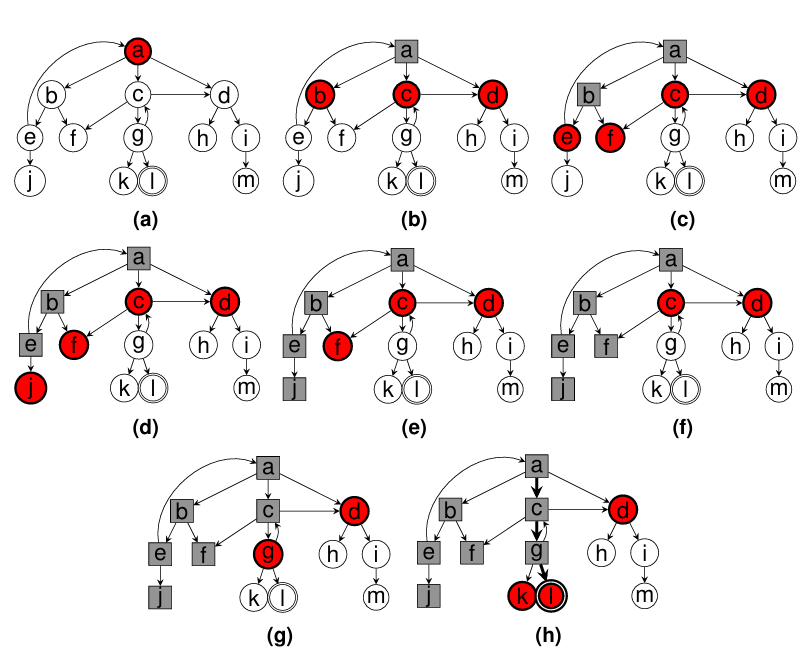
\includegraphics[width=0.8\textwidth]{./imgs/dfs.png}
	\caption{Depth First Search}
\end{figure}

\subsubsection{Pseudocode}
\begin{algorithm}[H]
	\caption{Depth First Search (\textit{state, maxdepth, maxtimeout})}
	\label{alg:dfs}
	\begin{algorithmic}[1]
	\State stack $\gets$ starting position of Sokoban
	\While {stack is not empty}
		\If {Ares crates on target}
			\State break
		\Else
			\If {Is deadlock or depth $\geq$ maxdepth or time $\geq$ maxtimeout}
				\State pick next solution
			\Else
				\State Get valid moves for Sokoban
				\ForAll {move}
					\State Find next state
					\State Put it in stack
				\EndFor
			\EndIf
		\EndIf
	\EndWhile
	\State \Return moves
	\end{algorithmic}
\end{algorithm}

\subsubsection{Implementation}

\subsubsection{Time and Space Complexity}